\chapter{Enterprise Service Bus}
\label{cha:esb}
An Enterprise Service Bus (ESB) is a architectural pattern which describes a distributed computing architecture, whereby distributed services are interacting with each other via the ESB. The ESB pattern if part of the Service Oriented Architecture Patterns (SOA).   
\\ \\
An ESB in the industry is mostly taken as a third party middleware, which provides features for implementing integrations with the Enterprise Integration Patterns (EI). Enterprises use third party middleware like JBoss Fuse for implementing integration services, which integrate external or internal services. JBoss Fuse is based on the Enterprise Application Platform (EAP), and bundles common frameworks used for integrations such as Camel, and is responsible for orchestration and mediation of the services.
\\ \\
The integration of internal as well as external services has become more important over time, especially with the appearance of cloud platforms like PaaS. Common ESB middleware on the market usually define the ESB as a single application, which contains all integration services, whereby all integration services share the same life-cycle. But the need for flexibility and shorter response times drives enterprises to split up their teams and integrations. This leads to separated services, which are managed as microservices, which have their own life cycle. De-coupling of teams leads to de-coupling of services, where the services need to provide a well defined and well managed public API\cite{Camel2015, RedHatAgileIntegration2017, EIP}.

\section{The need for an Enterprise Service Bus}
\label{sec:esb-need-for-esb}
Enterprises need an ESB to provide integrations between internal and external services or both, where the integration is meant to provide a business value for the enterprise. An integration of an external service could enhance the reach of a customer, who now could be able to consume external partner services via the enterprise provided infrastructure or product. In the digital age, it is normal to consume a digital service like Netflix, which runs a streaming service. Thus, integrations an enterprise has to provide and maintain will become more over time.

\section{Architecture}
\label{sec:esb-architecture}
Figure \vref{fig:esb-simple-architecture} illustrates the conceptional architecture of an ESB, which orchestrates and mediates integration services. A service can act either a producer service, which gets accessed by clients, or can act as a consumer service, which acts as the client for a producer service. The ESB is responsible for orchestration, mediation, security, transformation, routing and service discovery, whereby these aspects are covered by a ESB middleware provided frameworks and libraries. Additionally, an ESB middleware provides libraries which help to implement Service Components under consideration of the SOA and EI Patterns\cite{EsbSoa2018, MediationESB2005}.

\begin{figure}[htbp]
	\centering
	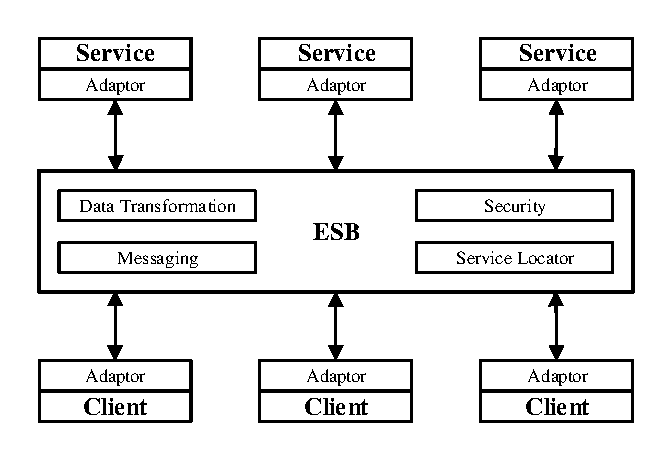
\includegraphics[scale=1]{images/esb-simple-architecture.pdf}
	\caption{Architecture of an ESB}
	\label{fig:esb-simple-architecture}
\end{figure} 

\begin{figure}[htbp]
	\centering
	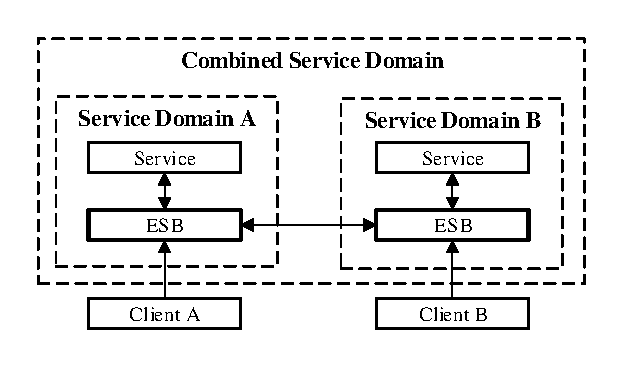
\includegraphics[scale=1]{images/esb-bidirectional-integration.pdf}
	\caption{Architecture of a bi-directional enterprise integration}
	\label{fig:esb-bidirectional-integration}
\end{figure} 

Figure \vref{fig:esb-bidirectional-integration} illustrates a bi-directional integration of services between two partner enterprises, whereby each integrated service is allowed to be consumed by the partner's customers, but only if the service is accessed via the partner's infrastructure. The ESB of the enterprises integrate the partner's provided services into their service domain, which can be accessed by their customers. For instance, an IP-TV provider can be integrated by an Internet Service-Provider (ISP), to provide Internet TV to their customers. 

\section{ESB with EAP}
\label{sec:esb-as-software}
An ESB is an architectural pattern for a distributed system, and has been implemented in software to provide an integration platform to developers, so that they can implement integration services under the consideration of the EAI patterns. Before the appearance of cloud platforms like PaaS, ESB implementations used existing platforms such as JBoss EAP, OSGI or Karaf for the service orchestration and mediation. In case of JBoss EAP, the platform provides all libraries and frameworks developers need for implementing an integration service. Commonly, the integration services are managed within a single application, which represents ESB. This is a monolithic approach of organizing integration services, but has the advantage that the management of the services is easier, because the source code is not separated, and therefore the implementations of all services needs to be consistent at compile time. Figure \vref{fig:esb-software-architecture} illustrates the monolithic organization of the integration services within a single ESB application, which is hosted on JBoss EAP.

\begin{figure}[htbp]
	\centering
	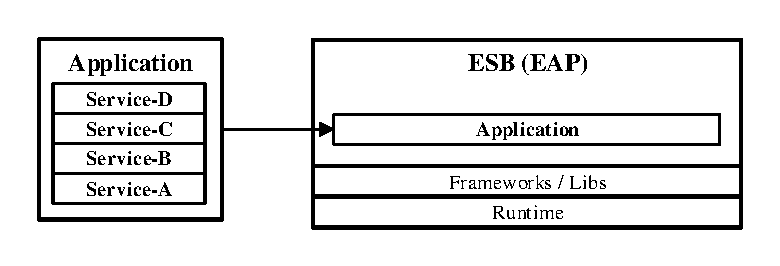
\includegraphics[scale=1]{images/esb-software-architecture.pdf}
	\caption{ESB running on EAP}
	\label{fig:esb-software-architecture}
\end{figure} 

With the appearance of cloud platforms such as PaaS, the cloud can now take over the mediation, orchestration and security aspects of an ESB. The integration services can be completely separated and de-coupled from each other, designed as microservices with their own life-cycle, and be managed by the cloud platform. Additionally, the integration services are hosted in a clustered infrastructure, which allows them to be distributed among multiple nodes, which increases fail over security. The new term for this kind of ESB is IPaaS, whereby the ESB is represented by an PaaS platform such as Openshift, which provides additional tooling for implementing integration services\cite{iPaaSP12015, iPaaSP22015}.

\section{ESB with Openshift}
\label{sec:esb-as-cloud}
With the appearance and general availability of cloud platforms like PaaS, it is possible now to move an ESB into the cloud, whereby the cloud platform takes over some aspects of the ESB middleware such as mediation and orchestration. A main problem of existing ESB implementations is the fact, that all integration services are managed within a single application, with one release version, and a shared life-cycle. If the ESB is an cloud platform, the integration services have to be implemented as separated services, which forces developers to separate their integration services into separate code bases, and to provide a proper designed and managed public API for their services. Figure \vref{fig:esb-cloud-architecture} illustrates the integration services of an ESB application, which runs on Openshift.

\begin{figure}[htbp]
	\centering
	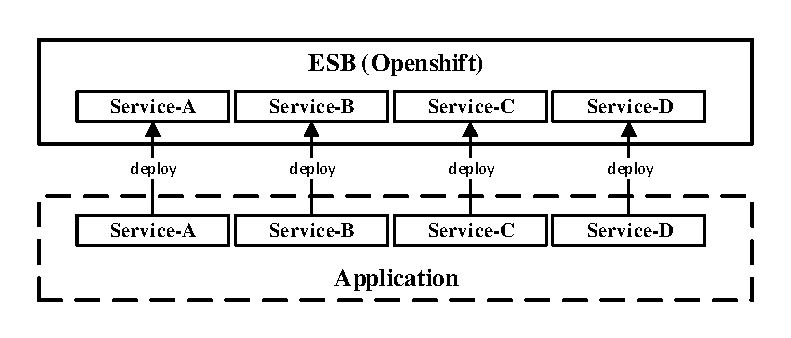
\includegraphics[scale=1]{images/esb-cloud-architecture.pdf}
	\caption{ESB application architecture with microservices}
	\label{fig:esb-cloud-architecture}
\end{figure} 

As discussed in the introduction of this chapter, enterprises need to separate their integrations and teams, to be faster and more responsive to business changes. Therefore, the microservice architecture, which is necessary when the ESB is represented by a cloud platform, can help enterprises to become more flexible.

\section{Integration example}
\label{sec:esb-integration-example}
This section will discuss an integration examples, and how it would have been designed as part of a monolithic ESB application. The integration discussed in this chapter is the base for the prototype of this thesis, which is specified in Chapter \vref{cha:esboc}. Figure \vref{fig:esb-design-services} illustrates the integration example, contained services and involved service domains. The integration service integrates an external database with an internal application, which is consumed by a public client. How the database is allowed to be accessed, is implemented in the integration service, which is the only service allowed to communicate with the external located database.
\newpage

\begin{figure}[htbp]
	\centering
	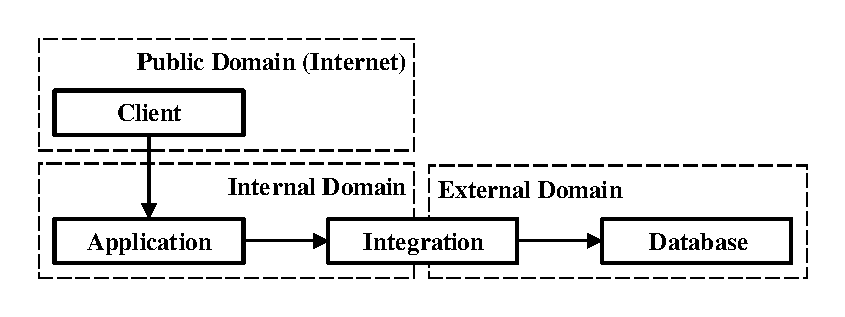
\includegraphics[scale=1]{images/esb-integration-example.pdf}
	\caption{Integration Service-Domains}
	\label{fig:esb-design-services}
\end{figure}

Figure \vref{fig:esb-design-sca} illustrates the design of the integration in an monolithic ESB application, with the use of Service Component Architecture (SCA). A service within the ESB application is represented by a service component, which exposes consumable services (\mentionedtext{Service}) and is connected to other services or external systems (\mentionedtext{Reference}). 

\begin{figure}[htbp]
	\centering
	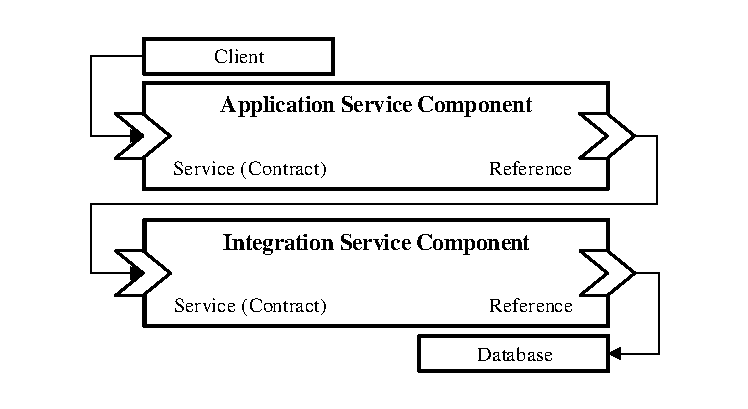
\includegraphics[scale=1]{images/esb-sca-example.pdf}
	\caption{Integration Services with SCA}
	\label{fig:esb-design-sca}
\end{figure}
  
ESB middleware, such as JBoss Fuse provides frameworks and libraries, which implement the SCA patterns and provide a lightweight way of implementing service components. The service component orchestration, mediation is done by the ESB middleware. Additionally, the ESB middleware provides bindings for commonly used technologies such as REST or SOAP, which can be applied to services and references. Thus, the developers don't have to setup for instance a REST Server or REST Client anymore, but only need to provide the service contract and connection settings\cite{MicroSoa2008, Richards2015}.\\

The following chapter will specify the prototype based on the introduced integration example, and will show that an ESB can be implemented on Openshift.